%%============================================================================
%%  CSEE W4823 Advanced Logic Design -- Individual Project, Report #1
%%
%%  Compiles as-is on Overleaf: upload this file plus the figures/ folder.
%%  Template: IEEE conference (double column), pdflatex.
%%============================================================================
\documentclass[conference]{IEEEtran}

\usepackage[T1]{fontenc}
\usepackage[utf8]{inputenc}
\usepackage{amsmath,amssymb}
\usepackage{graphicx}
\usepackage{booktabs}
\usepackage{array}
\usepackage{algorithm}
\usepackage{algpseudocode}
\usepackage{url}
\usepackage[hidelinks]{hyperref}

\graphicspath{{figures/}}

% IEEEtran already sets \bfseries etc.; a few small conveniences
\newcommand{\qf}[2]{Q#1.#2}
\renewcommand{\algorithmicrequire}{\textbf{Input:}}
\renewcommand{\algorithmicensure}{\textbf{Output:}}

\begin{document}

\title{Architecture and Self-Checking Verification of a\\
100\,MS/s 64-Tap FIR Filter Core in Q1.15 Fixed Point}

\author{\IEEEauthorblockN{Yanxiang Zhu}
\IEEEauthorblockA{Department of Electrical Engineering\\
Columbia University, New York, NY\\
\url{yz5479@columbia.edu}}}

\maketitle

\begin{abstract}
This report defines the architecture of a 64-tap FIR filter core that must
sustain 100\,MS/s with 16-bit $\qf{1}{15}$ inputs and coefficients and a 16-bit
$\qf{7}{9}$ output, while two asynchronous clocks close the input interface.
We first settle the numerical design: a word-length sweep against a
binary32 golden model shows the output format itself already sets a
$0.0029\,\%$ NRMSE floor, so the internal datapath can be narrowed to 20-bit
$\qf{2}{18}$ products and a 32-bit accumulator at no measurable accuracy cost.
We then choose eight parallel multipliers clocked at 800\,MHz, and solve the
resulting sample-window problem with a \emph{rotating} banked register file
that keeps the read cost at one port per bank.
The report closes with the pseudocode, the ASM chart, the datapath block
diagram and the interface specification of every block, together with a
self-checking testbench whose golden model, stimulus and error accounting are
already operational.
\end{abstract}

\begin{IEEEkeywords}
FIR filter, fixed point, Q1.15, clock-domain crossing, register file, ASM chart,
self-checking testbench, NRMSE
\end{IEEEkeywords}

%%============================================================================
\section{Introduction}
%%============================================================================

The project asks for a 64-tap finite-impulse-response filter implemented as a
hardware core. Each clock the core consumes one 16-bit $\qf{1}{15}$ sample,
multiplies it by 64 $\qf{1}{15}$ coefficients, accumulates, and produces one
16-bit $\qf{7}{9}$ output, sustaining 100 million samples per second. The
coefficients are preloaded through a single write port; the core runs on a
second clock whose frequency is ours to choose and which is
\emph{phase-unsynchronised} with the input clock. Because the specification
fixes the throughput, the graded figure of merit
\begin{equation}
  \mathrm{FoM} \;=\; \frac{\text{Throughput}}{\text{Energy/sample} \times \text{Area}}
\end{equation}
leaves only energy and area as free variables
\cite{lec}. Report~\#1 fixes the algorithm, the arithmetic and the
micro-architecture; the three later reports build the ALU, the memories and
the assembled core behind the interfaces defined here.

Section~\ref{sec:num} settles the fixed-point formats, Section~\ref{sec:arch}
the micro-architecture, Section~\ref{sec:control} the control path,
Section~\ref{sec:tb} the verification environment, and
Section~\ref{sec:spec} collects the per-block interface requirements.

%%============================================================================
\section{Numerical Design}\label{sec:num}
%%============================================================================

\subsection{Formats and the error floor}

Inputs and coefficients are signed $\qf{1}{15}$: one sign bit, one integer bit
and fifteen fractional bits, covering $[-1,+1)$. A 16$\times$16 product is
exact in $\qf{2}{30}$, and 64 of them are accumulated before the result is
rounded back to $\qf{7}{9}$. Both the golden model and the DUT operate on the
\emph{same} quantised words, so the measured error isolates fixed-point
truncation rather than input quantisation.

The important observation is that the output format, not the datapath, sets
the accuracy floor. With $\mathrm{LSB} = 2^{-9}$ the output quantisation noise
has RMS $\mathrm{LSB}/\sqrt{12} \approx 5.6\times10^{-4}$, and the measured
dynamic range of $y$ over random $\qf{1}{15}$ coefficient sets is
$\mathrm{span}(y)\approx 20.1$. The resulting floor,
$5.6\times10^{-4}/20.1 \approx 0.0028\,\%$. The datapath lands at
$0.0029\,\%$: within one measurement of the floor, and three orders of
magnitude inside the course target.

\subsection{Word-length sweep}

Table~\ref{tab:pw} sweeps the product width with the full core
(10\,000 samples, random $\qf{1}{15}$ stimulus, binary32 golden reference).
Rounding is round-half-up on the discarded product bits.

\begin{table}[t]
\centering
\caption{Output accuracy versus product word length. The error is flat down to
16 bits, i.e.\ the datapath is not the limiting factor.}
\label{tab:pw}
\begin{tabular}{@{}lccrr@{}}
\toprule
Product & Acc. & avg NRMSE & worst NRMSE & max err.\\
format  & width & (\%)     & (\%)        & (LSB)\\
\midrule
$\qf{2}{14}$ (16 b) & 32 b & 0.0030 & 0.0077 & 0.77\\
$\qf{2}{18}$ (20 b) & 32 b & 0.0029 & 0.0051 & 0.51\\
$\qf{2}{22}$ (24 b) & 32 b & 0.0029 & 0.0050 & 0.50\\
$\qf{2}{30}$ (32 b) & 40 b & 0.0029 & 0.0050 & 0.50\\
\bottomrule
\end{tabular}
\end{table}

Two conclusions follow. First, the worst-case error of the 20-bit design is
0.51 LSB of the output format: the datapath sits exactly on the output
quantisation floor, so buying internal precision buys nothing. Second, the
course target for NRMSE is a low single-digit percentage; the design is three
orders of magnitude inside it. Precision is therefore \emph{not} a design
variable here -- area and energy are. We fix the baseline at 20-bit
$\qf{2}{18}$ products with a 32-bit accumulator, and keep the product width as
a sweep parameter for the ALU report.

Truncation must be accompanied by rounding. A separate model of the same
datapath with plain truncation (round toward $-\infty$) accumulates a
measurable dc offset of $-0.0083\,\%$ on this coefficient set and doubles the
worst-case error; round-half-up removes the offset entirely
($+0.0001\,\%$).

\subsection{Range}

Since $|x|<1$ and $|b|<1$, $|y|<64$ holds for any coefficient set, so a
$\qf{7}{9}$ word never overflows: the extreme input
$x=b=32767$ gives $y = 63.996$. The saturator is therefore defensive only;
Section~\ref{sec:tb} verifies it by forcing the internal value past the rail
rather than by searching for an input that reaches it.

%%============================================================================
\section{Micro-architecture}\label{sec:arch}
%%============================================================================

\subsection{How many multipliers}

64 multiply-accumulates must complete inside one 10\,ns sample period. The
number of parallel MACs $P$ and the core clock $f_2$ trade against each other,
$f_2 = P \times 100\,\mathrm{MHz}$:

\begin{table}[t]
\centering
\caption{Parallelism versus clock. Energy per sample for the arithmetic itself
is fixed at 64 MACs; only the clock network and the adder tree scale with $P$.}
\label{tab:p}
\begin{tabular}{@{}lcl@{}}
\toprule
$P$ & $f_2$ & remark\\
\midrule
1  & 6.4\,GHz & not implementable\\
4  & 1.6\,GHz & timing critical\\
\textbf{8} & \textbf{800\,MHz} & \textbf{baseline: fewest multipliers}\\
16 & 400\,MHz & area for timing margin\\
32 & 200\,MHz & multiplier count explodes\\
\bottomrule
\end{tabular}
\end{table}

We take $P=8$, $f_2=800\,\mathrm{MHz}$: eight MACs, eight cycles per output,
one sample accepted per eight cycles. This minimises the multiplier count,
which dominates both area and switching energy. Because one cycle is 1.25\,ns
and a 16$\times$16 multiply truncated to $\qf{2}{18}$ costs roughly
0.6--0.7\,ns in a modern node, the datapath is pipelined into a multiplier
stage and an adder-tree stage, so each stage gets its own 1.25\,ns budget.
Latency is unconstrained by the specification, which makes this split free.

\begin{figure*}[t]
\centering
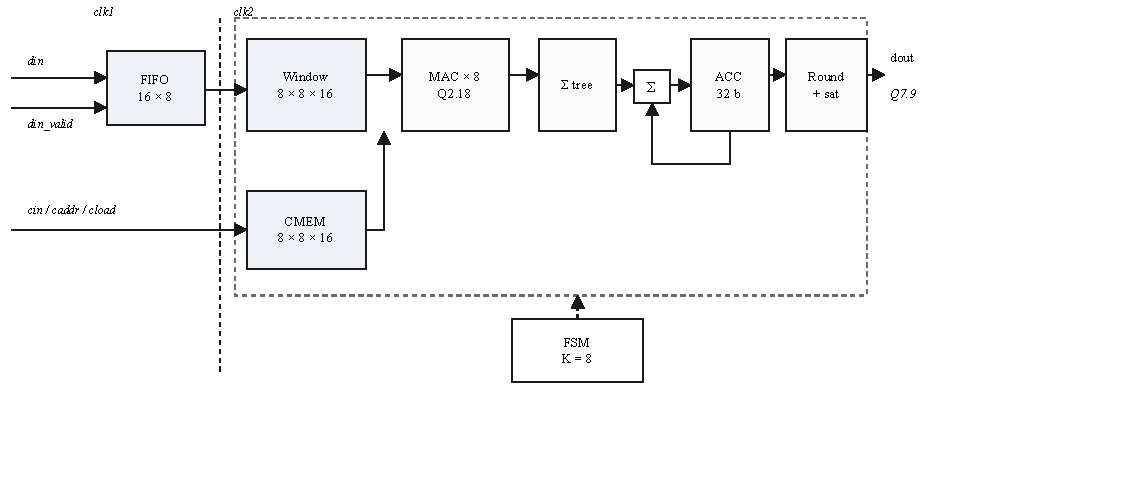
\includegraphics[width=\textwidth]{dut-block.pdf}
\caption{Block diagram of the DUT. The dashed vertical line is the
asynchronous clock boundary; the dashed box marks the blocks sequenced by the
controller. Eight MACs consume one tap group $(x_g,c_g)$ per cycle; the
accumulator feeds back into the adder, and the final stage rounds and saturates
to $\qf{7}{9}$.}
\label{fig:block}
\end{figure*}

\subsection{The sample window problem}

The core needs the last 64 samples, and at cycle $j$ the eight multipliers need
taps $i = p + 8j$ for $p=0\ldots7$. A plain 64-entry shift register would
require eight read ports, or a 64:1 multiplexer in front of every multiplier.

We instead bank the window: bank $p$ holds the samples of tap group $p$, so at
step $j$ every bank reads its own entry $j$ and one read port per bank
suffices (Fig.~\ref{fig:map}). The subtlety is that a new sample still shifts
all 64 delays by one, which in the banked layout means \emph{every} bank would
have to move. The trick is to rotate the \emph{role} of the banks instead of
their contents: the rotation index decrements on every accepted sample, so
taps keep pointing at the right bank, and only the one bank that is being
retired from group 7 to group 0 is physically rewritten -- it shifts down by
one entry and takes the new sample at entry 0. The other seven banks keep
their data untouched. The rotation index is a read-address offset, i.e.\
free in hardware.

The coefficient memory uses the identical layout, which requires transposing
the preload address: the externally supplied index $i$ is stored at
bank $(i \bmod 8)$, entry $(i \,\mathrm{div}\, 8)$, so that group $j$
presents $b[p+8j]$ on port $p$. Multiplier $p$ therefore reads exactly one
window word and one coefficient word per cycle, both from entry $j$ of bank
$p$.

\begin{figure}[t]
\centering
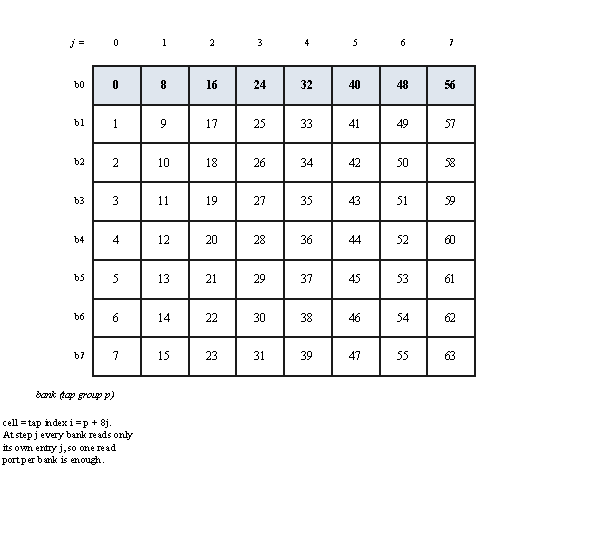
\includegraphics[width=\columnwidth]{tap-map.pdf}
\caption{Tap index map. Cell $(b,j)$ is the tap that bank $b$ supplies at step
$j$; the highlighted row is the bank rewritten on the current sample. Reading
one entry per bank per step is what keeps the port count at one.}
\label{fig:map}
\end{figure}

\subsection{Read/write hazard}

The accepted sample is written at the same edge at which group 0 is read, and
the bank being written is precisely the bank that serves group 0. Exactly one
tap collides -- tap $p=0$ of group $j=0$ -- and the value it needs is the
incoming sample itself, so a single 2:1 write-through bypass on that one tap
resolves the hazard. Entries $j\ge 1$ are read on later cycles and are
therefore never in conflict.

%%============================================================================
\section{Control}\label{sec:control}
%%============================================================================

The controller is a small FSM with one state per tap group. Because the
arithmetic is pipelined by one cycle, group $j$ is issued in cycle $j$ and
consumed in cycle $j+1$; group $K-1$ is therefore consumed exactly when the
next sample is accepted, which keeps the period at $K$ cycles.

\begin{figure}[t]
\centering
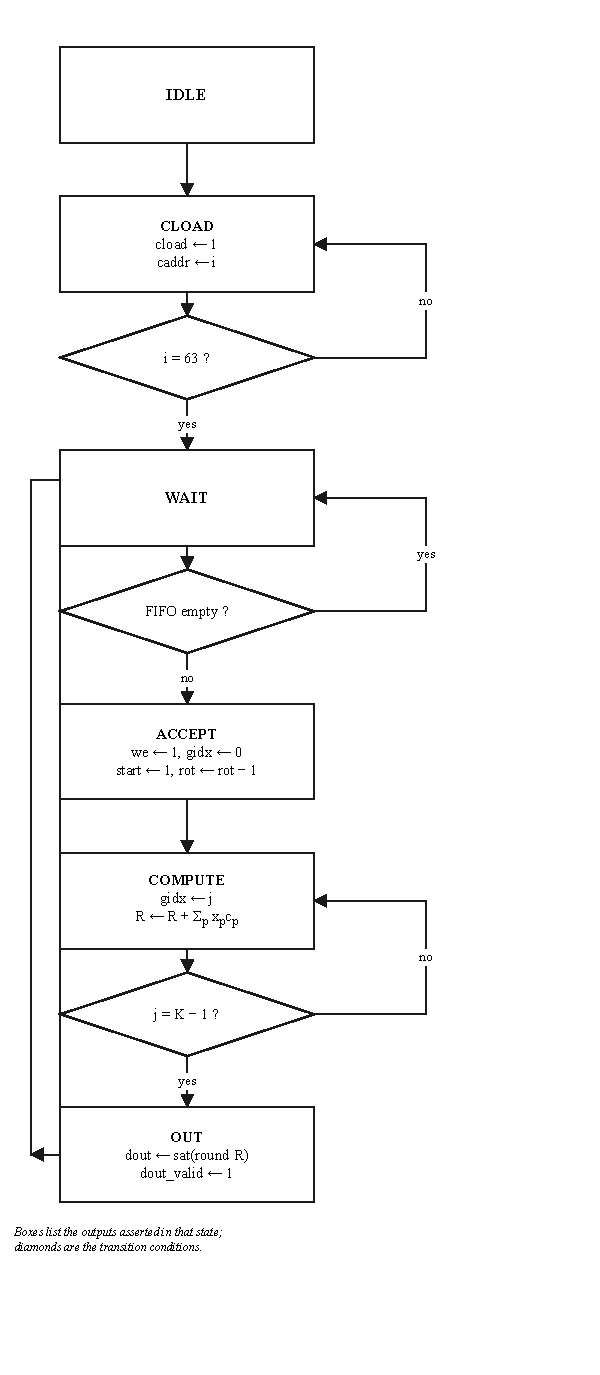
\includegraphics[width=\columnwidth]{asm-chart.pdf}
\caption{ASM chart. Loop-backs run in the right-hand corridor, the single
return path from \textsc{Out} to \textsc{Wait} in the left-hand one.}
\label{fig:asm}
\end{figure}

\begin{algorithm}[t]
\caption{DUT operation ($K=8$, one iteration per \texttt{clk2})}
\label{alg:dut}
\begin{algorithmic}[1]
\Require coefficient words $C_{in}$, index $i$, strobe \texttt{cload};
         input samples $x[n]$ from the asynchronous FIFO
\Ensure  output words $y[n]$ in $\qf{7}{9}$ with valid flag
\Statex
\Statex \emph{coefficient preload, 64 cycles}
\For{$i \gets 0$ \textbf{to} 63}
  \State $C[i \bmod 8][i \,\mathrm{div}\, 8] \gets C_{in}$ \textbf{if} \texttt{cload}
\EndFor
\Statex
\Statex \emph{main loop}
\Loop
  \If{$g = 0$}
    \If{holding register full}
      \State $q \gets (\mathit{rot} - 1) \bmod 8$
      \State $W[q][0] \gets x[n]$
      \State \textbf{for} $j \gets 7$ \textbf{down to} 1 \textbf{do}
             $W[q][j] \gets W[q][j-1]$
      \State $\mathit{rot} \gets q$; \quad $R \gets 0$
      \State $g \gets 1$
    \EndIf
  \Else
    \State \textbf{for} $p \gets 0$ \textbf{to} 7 \textbf{do}
           $W_p \gets W[(p+\mathit{rot}) \bmod 8]$
    \State $R \gets R + \sum_{p=0}^{7} \qf{2}{18}(W_p[g] \cdot C[p][g])$
    \If{$g = 7$}
      \State $y[n] \gets \mathrm{sat}\!\left(\mathrm{round}_{9}(R)\right)$; \quad valid
      \State $g \gets 0$
    \Else
      \State $g \gets g + 1$
    \EndIf
  \EndIf
\EndLoop
\end{algorithmic}
\end{algorithm}

\subsection{Clock-domain crossing}

The two clocks are specified to be phase-unsynchronised, so the sample path
crosses domains through a dual-clock FIFO of depth 8: gray-coded read and
write pointers, two flip-flop synchronisers in each direction, and full/empty
flags evaluated on the registered pointers so that no flag feeds back
combinationally into its own next-state value. The full flag inverts the two
most significant gray bits, since a pointer exactly $2^{3}$ ahead differs in
exactly those two bits; inverting only the most significant bit reports
\emph{full while empty} and silently discards every word that arrives.

A one-word prefetch stage sits between the FIFO and the window. It holds the
next sample while the current one is being processed, so the two-cycle pointer
synchronisation latency never turns into a lost slot; at $f_2 = 8f_1$ there is
no rate margin, and without the prefetch a bursty input slowly fills the FIFO.

%%============================================================================
\section{Verification Environment}\label{sec:tb}
%%============================================================================

\subsection{Golden model}

The golden block is a binary32 (\texttt{shortreal}) implementation of the same
convolution. It lives in the testbench and is never synthesised; its only job
is to produce the numerically correct answer for the \emph{quantised} input
words, so that the measured difference is purely the DUT's own truncation.
Using binary32 rather than double is deliberate: the mantissa of a float32 is
$2^{-24}$, four orders of magnitude finer than the $\qf{7}{9} \sim 2^{-9}$
output grid, so it cannot mask a datapath error.

\subsection{Stimulus}

The testbench drives both clocks from one time base with an arbitrary phase
offset (default 0.31\,ns, swept 0--1.1\,ns), resets the core, preloads 64
random $\qf{1}{15}$ coefficients one word per core cycle through
\texttt{cin}/\texttt{caddr}/\texttt{cload}, and then streams
$10^4$ uniformly distributed $\qf{1}{15}$ samples at 100\,MS/s. The value
$-1.0$ (code \texttt{0x8000}) is excluded because it lies outside the
representable range. Optional plusargs add idle cycles to the stream
(\texttt{+GAPS}) to exercise FIFO elasticity, and change the seed
(\texttt{+SEED}) or the phase (\texttt{+PHASE}).

\subsection{Checking and metrics}

Every output is compared with the golden value of the same index. The
scoreboard accumulates the squared error, tracks $\min y$ and $\max y$, and
reports
\begin{equation}
  \mathrm{NRMSE}_{\mathrm{avg}} = \frac{\sqrt{\overline{e^2}}}{y_{\max}-y_{\min}},
\end{equation}
\begin{equation}
  \mathrm{NRMSE}_{\mathrm{wc}}  = \frac{\max |e|}{y_{\max}-y_{\min}},
\end{equation}
which is the definition used in the course. Output count is checked as well,
so a dropped sample fails the test even if the values that did appear are
correct.

\begin{figure}[t]
\centering
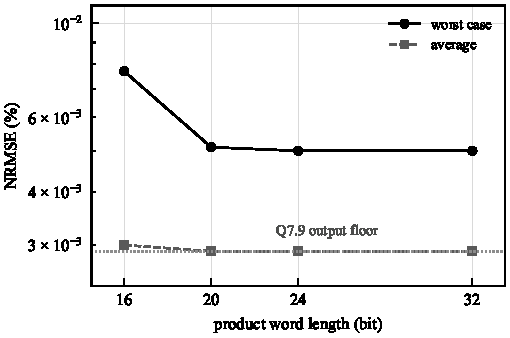
\includegraphics[width=\columnwidth]{accuracy.pdf}
\caption{Measured NRMSE against product word length, with the output
quantisation floor for reference. The curve is flat: the format of $y$
decides the error, not the internal precision.}
\label{fig:acc}
\end{figure}

\subsection{Current status}

The environment is operational against a behavioural reference model of the
specified arithmetic and already produces the numbers of
Table~\ref{tab:pw} and Fig.~\ref{fig:acc}: average NRMSE $0.0029\,\%$,
worst case $0.0051\,\%$, peak error 0.51\,LSB, over 10\,000 samples. Across
five stimulus seeds the worst case stays within $0.0047$--$0.0052\,\%$, and
sweeping the clk2 phase over $0$--$1.1$\,ns leaves the figures bit-identical,
which is the direct evidence that the asynchronous interface is transparent.
The same testbench, unchanged, is the acceptance test for the assembled core
in Report~\#4.

%%============================================================================
\section{Block Specifications}\label{sec:spec}
%%============================================================================

Table~\ref{tab:spec} is the interface contract between the blocks. It is what
Reports \#2 and \#3 implement against, and what Report~\#4 instantiates
unchanged.

\begin{table*}[t]
\centering
\caption{Required specification of each datapath block.}
\label{tab:spec}
\renewcommand{\arraystretch}{1.15}
\begin{tabular}{@{}p{1.95cm}p{2.15cm}p{1.2cm}p{2.3cm}p{2.25cm}p{4.35cm}@{}}
\toprule
Block & Function & Clock & Ports & Size / width & Notes\\
\midrule
Synchroniser & clock-domain crossing & clk1 / clk2 &
1 write (clk1), 1 read (clk2) & 8 $\times$ 16 b, 3-bit pointers &
gray-coded pointers, two-flop synchronisers, registered full/empty; must never
assert full below depth, must not drop words under a bursty input\\
\addlinespace
Sample window & last 64 samples & clk2 &
1 write, 8 read (one per bank) & 64 $\times$ 16 b, 8 banks $\times$ 8 entries &
rotating register file; only the retired bank is rewritten; one 2:1
write-through bypass on tap 0 of group 0\\
\addlinespace
CMEM & 64 coefficients & clk2 &
1 write, 8 read & 64 $\times$ 16 b, 8 banks $\times$ 8 entries &
address transposed on preload ($i \mapsto (i\bmod 8, i\,\mathrm{div}\,8)$);
64 cycles to load\\
\addlinespace
MAC array & product formation & clk2 &
8 in, 8 out & 8 $\times$ (16$\times$16), 20 b $\qf{2}{18}$ &
round-half-up on the discarded product bits; registered output of stage 1\\
\addlinespace
Adder tree & group sum & clk2 & 8 in, 1 out &
3 levels, 23 b & 3-bit growth, sign-extended into the accumulator\\
\addlinespace
Accumulator & 64-tap sum & clk2 & 1 in, 1 out &
32 b $\qf{2}{18}$ & 26 b required, 6 b head-room; cleared on the last group\\
\addlinespace
Round / saturate & format conversion & clk2 & 1 in, 1 out &
32 b $\to$ 16 b $\qf{7}{9}$ & round-half-up, saturating; saturator provably
unreachable for $|x|<1$, kept as a guard\\
\addlinespace
Controller & sequencing & clk2 & 8 states &
3-bit group counter & one state per tap group; stalls in state 0 when no sample
is ready\\
\bottomrule
\end{tabular}
\end{table*}

%%============================================================================
\section{Conclusion}\label{sec:concl}
%%============================================================================

The numerical study shows that a $\qf{2}{18}$ product with a 32-bit
accumulator already sits on the $\qf{7}{9}$ output quantisation floor, so the
architecture is free to optimise area and energy rather than precision. Eight
multipliers at 800\,MHz satisfy the throughput with the fewest multipliers,
and the rotating banked window turns what would be an eight-port,
1024-bit register file into eight single-port banks plus an address rotation.
The control path is a nine-state ASM chart, and the asynchronous interface is
closed with a dual-clock FIFO plus a one-word prefetch stage.

Reports \#2--\#4 implement the ALU, the memories and the assembled core
against the interfaces of Table~\ref{tab:spec}, and replace the behavioural
reference by synthesised RTL behind the same testbench.

\begin{thebibliography}{1}
\bibitem{lec}
CSEE~W4823, \emph{Advanced Logic Design}, lecture notes and project
specification, Columbia University, Fall 2026.
\end{thebibliography}

\end{document}
